
\documentclass[letterpaper,hide notes,xcolor={table,svgnames},10pt]{beamer}
\def\showexamples{t}


%\usepackage[svgnames]{xcolor}

%% Demo talk
%\documentclass[letterpaper,notes=show]{beamer}

\usecolortheme{crane}
\setbeamertemplate{navigation symbols}{}

\usetheme{MyPittsburgh}
%\usetheme{Frankfurt}

%\usepackage{tipa}

\usepackage{hyperref}
\usepackage{graphicx,xspace}
\usepackage[normalem]{ulem}
\usepackage{multicol}
\usepackage{amsmath,amssymb,amsthm,graphicx,xspace}
\newcommand\SF[1]{$\bigstar$\footnote{SF: #1}}

\usepackage[default]{sourcesanspro}
\usepackage[T1]{fontenc}
\usepackage[scaled]{beramono}
\usepackage{tikzpagenodes}

\newcounter{tmpnumSlide}
\newcounter{tmpnumNote}


% old question code
%\newcommand\question[1]{{$\bigstar$ \small \onlySlide{2}{#1}}}
% \newcommand\nquestion[1]{\ifdefined \presentationonly \textcircled{?} \fi \note{\par{\Large \textbf{?}} #1}}
% \newcommand\nanswer[1]{\note{\par{\Large \textbf{A}} #1}}


 \newcommand\mnote[1]{%
   \addtocounter{tmpnumSlide}{1}
   \ifdefined\showcues {~\tiny\fbox{\arabic{tmpnumSlide}}}\fi
   \note{\setlength{\parskip}{1ex}\addtocounter{tmpnumNote}{1}\textbf{\Large \arabic{tmpnumNote}:} {#1\par}}}

\newcommand\mmnote[1]{\note{\setlength{\parskip}{1ex}#1\par}}

%\newcommand\mnote[2][]{\ifdefined\handoutwithnotes {~\tiny\fbox{#1}}\fi
% \note{\setlength{\parskip}{1ex}\textbf{\Large #1:} #2\par}}

%\newcommand\mnote[2][]{{\tiny\fbox{#1}} \note{\setlength{\parskip}{1ex}\textbf{\Large #1:} #2\par}}

\newcommand\mquestion[2]{{~\color{red}\fbox{?}}\note{\setlength{\parskip}{1ex}\par{\Large \textbf{?}} #1} \note{\setlength{\parskip}{1ex}\par{\Large \textbf{A}} #2\par}\ifdefined \presentationonly \pause \fi}

\newcommand\blackboard[1]{%
\ifdefined   \showblackboard
  {#1}
  \else {\begin{center} \fbox{\colorbox{blue!30}{%
         \begin{minipage}{.95\linewidth}%
           \hspace{\stretch{1}} Some space intentionally left blank; done at the blackboard.%
         \end{minipage}}}\end{center}}%
         \fi%
}

\newcommand{\Rplus}{\protect\hspace{-.1em}\protect\raisebox{.35ex}{\small{\small\textbf{+}}}}
\newcommand{\CPP}{\mbox{C\Rplus\Rplus}\xspace}

%\newcommand\q{\tikz \node[thick,color=black,shape=circle]{?};}
%\newcommand\q{\ifdefined \presentationonly \textcircled{?} \fi}

\usepackage{listings,listings-rust}
\lstset{basicstyle=\footnotesize\ttfamily,
	breaklines=true,
	aboveskip=15pt,
  	belowskip=15pt,
	frame=lines,
	numbers=left, basicstyle=\scriptsize, numberstyle=\tiny, stepnumber=0, numbersep=2pt
}

\usepackage{siunitx}
\newcommand\sius[1]{\num[group-separator = {,}]{#1}\si{\micro\second}}
\newcommand\sims[1]{\num[group-separator = {,}]{#1}\si{\milli\second}}
\newcommand\sins[1]{\num[group-separator = {,}]{#1}\si{\nano\second}}
\sisetup{group-separator = {,}, group-digits = true}

%% -------------------- tikz --------------------
\usepackage{tikz}
\usetikzlibrary{positioning}
\usetikzlibrary{arrows,backgrounds,automata,decorations.shapes,decorations.pathmorphing,decorations.markings,decorations.text,decorations.pathreplacing}

\tikzstyle{place}=[circle,draw=blue!50,fill=blue!20,thick, inner sep=0pt,minimum size=6mm]
\tikzstyle{transition}=[rectangle,draw=black!50,fill=black!20,thick, inner sep=0pt,minimum size=4mm]

\tikzstyle{block}=[rectangle,draw=black, thick, inner sep=5pt]
\tikzstyle{bullet}=[circle,draw=black, fill=black, thin, inner sep=2pt]

\tikzstyle{pre}=[<-,shorten <=1pt,>=stealth',semithick]
\tikzstyle{post}=[->,shorten >=1pt,>=stealth',semithick]
\tikzstyle{bi}=[<->,shorten >=1pt,shorten <=1pt, >=stealth',semithick]

\tikzstyle{mut}=[-,>=stealth',semithick]

\tikzstyle{treereset}=[dashed,->, shorten >=1pt,>=stealth',thin]

\usepackage{ifmtarg}
\usepackage{xifthen}
\makeatletter
% new counter to now which frame it is within the sequence
\newcounter{multiframecounter}
% initialize buffer for previously used frame title
\gdef\lastframetitle{\textit{undefined}}
% new environment for a multi-frame
\newenvironment{multiframe}[1][]{%
\ifthenelse{\isempty{#1}}{%
% if no frame title was set via optional parameter,
% only increase sequence counter by 1
\addtocounter{multiframecounter}{1}%
}{%
% new frame title has been provided, thus
% reset sequence counter to 1 and buffer frame title for later use
\setcounter{multiframecounter}{1}%
\gdef\lastframetitle{#1}%
}%
% start conventional frame environment and
% automatically set frame title followed by sequence counter
\begin{frame}%
\frametitle{\lastframetitle~{\normalfont(\arabic{multiframecounter})}}%
}{%
\end{frame}%
}
\makeatother

\makeatletter
\newdimen\tu@tmpa%
\newdimen\ydiffl%
\newdimen\xdiffl%
\newcommand\ydiff[2]{%
    \coordinate (tmpnamea) at (#1);%
    \coordinate (tmpnameb) at (#2);%
    \pgfextracty{\tu@tmpa}{\pgfpointanchor{tmpnamea}{center}}%
    \pgfextracty{\ydiffl}{\pgfpointanchor{tmpnameb}{center}}%
    \advance\ydiffl by -\tu@tmpa%
}
\newcommand\xdiff[2]{%
    \coordinate (tmpnamea) at (#1);%
    \coordinate (tmpnameb) at (#2);%
    \pgfextractx{\tu@tmpa}{\pgfpointanchor{tmpnamea}{center}}%
    \pgfextractx{\xdiffl}{\pgfpointanchor{tmpnameb}{center}}%
    \advance\xdiffl by -\tu@tmpa%
}
\makeatother
\newcommand{\copyrightbox}[3][r]{%
\begin{tikzpicture}%
\node[inner sep=0pt,minimum size=2em](ciimage){#2};
\usefont{OT1}{phv}{n}{n}\fontsize{4}{4}\selectfont
\ydiff{ciimage.south}{ciimage.north}
\xdiff{ciimage.west}{ciimage.east}
\ifthenelse{\equal{#1}{r}}{%
\node[inner sep=0pt,right=1ex of ciimage.south east,anchor=north west,rotate=90]%
{\raggedleft\color{black!50}\parbox{\the\ydiffl}{\raggedright{}#3}};%
}{%
\ifthenelse{\equal{#1}{l}}{%
\node[inner sep=0pt,right=1ex of ciimage.south west,anchor=south west,rotate=90]%
{\raggedleft\color{black!50}\parbox{\the\ydiffl}{\raggedright{}#3}};%
}{%
\node[inner sep=0pt,below=1ex of ciimage.south west,anchor=north west]%
{\raggedleft\color{black!50}\parbox{\the\xdiffl}{\raggedright{}#3}};%
}
}
\end{tikzpicture}
}


%% --------------------

%\usepackage[excludeor]{everyhook}
%\PushPreHook{par}{\setbox0=\lastbox\llap{MUH}}\box0}

%\vspace*{\stretch{1}

%\setbox0=\lastbox \llap{\textbullet\enskip}\box0}

\setlength{\parskip}{\fill}

\newcommand\noskips{\setlength{\parskip}{1ex}}
\newcommand\doskips{\setlength{\parskip}{\fill}}

\newcommand\xx{\par\vspace*{\stretch{1}}\par}
\newcommand\xxs{\par\vspace*{2ex}\par}
\newcommand\tuple[1]{\langle #1 \rangle}
\newcommand\code[1]{{\sf \footnotesize #1}}
\newcommand\ex[1]{\uline{Example:} \ifdefined \presentationonly \pause \fi
  \ifdefined\showexamples#1\xspace\else{\uline{\hspace*{2cm}}}\fi}

\newcommand\ceil[1]{\lceil #1 \rceil}


\AtBeginSection[]
{
   \begin{frame}
       \frametitle{Outline}
       \tableofcontents[currentsection]
   \end{frame}
}



\pgfdeclarelayer{edgelayer}
\pgfdeclarelayer{nodelayer}
\pgfsetlayers{edgelayer,nodelayer,main}

\tikzstyle{none}=[inner sep=0pt]
\tikzstyle{rn}=[circle,fill=Red,draw=Black,line width=0.8 pt]
\tikzstyle{gn}=[circle,fill=Lime,draw=Black,line width=0.8 pt]
\tikzstyle{yn}=[circle,fill=Yellow,draw=Black,line width=0.8 pt]
\tikzstyle{empty}=[circle,fill=White,draw=Black]
\tikzstyle{bw} = [rectangle, draw, fill=blue!20, 
    text width=4em, text centered, rounded corners, minimum height=2em]
    
    \newcommand{\CcNote}[1]{% longname
	This work is licensed under the \textit{Creative Commons #1 3.0 License}.%
}
\newcommand{\CcImageBy}[1]{%
	\includegraphics[scale=#1]{creative_commons/cc_by_30.pdf}%
}
\newcommand{\CcImageSa}[1]{%
	\includegraphics[scale=#1]{creative_commons/cc_sa_30.pdf}%
}
\newcommand{\CcImageNc}[1]{%
	\includegraphics[scale=#1]{creative_commons/cc_nc_30.pdf}%
}
\newcommand{\CcGroupBySa}[2]{% zoom, gap
	\CcImageBy{#1}\hspace*{#2}\CcImageNc{#1}\hspace*{#2}\CcImageSa{#1}%
}
\newcommand{\CcLongnameByNcSa}{Attribution-NonCommercial-ShareAlike}

\newenvironment{changemargin}[1]{% 
  \begin{list}{}{% 
    \setlength{\topsep}{0pt}% 
    \setlength{\leftmargin}{#1}% 
    \setlength{\rightmargin}{1em}
    \setlength{\listparindent}{\parindent}% 
    \setlength{\itemindent}{\parindent}% 
    \setlength{\parsep}{\parskip}% 
  }% 
  \item[]}{\end{list}} 




\title{Lecture 17 --- Mostly Data Parallelism }

\author{Patrick Lam \\ \small \texttt{patrick.lam@uwaterloo.ca}}
\institute{Department of Electrical and Computer Engineering \\
  University of Waterloo}
\date{\today}


\begin{document}

\begin{frame}
  \titlepage

 \end{frame}


%%%%%%%%%%%%%%%%%%%%%%%%%%%%%%%%%%%%%%%%%%%%%%%%%%%%%%%%%%%%%%%%%%%%%%%%%%%%%%%%
\begin{frame}
  \frametitle{Data and Task Parallelism}

  
     \structure{Data parallelism} is performing \emph{the same} operations on
      different input.\\

     {\bf Example:} doubling all elements of an array.\\[1em]

     \structure{Task parallelism} is performing \emph{different} operations
      on different input.

    {\bf Example:} playing a video file: one thread decompresses
      frames, another renders.

  
\end{frame}
%%%%%%%%%%%%%%%%%%%%%%%%%%%%%%%%%%%%%%%%%%%%%%%%%%%%%%%%%%%%%%%%%%%%%%%%%%%%%%%%


\begin{frame}
\frametitle{You're Not Using Those Bytes, Are You?}

Consider the size of an \texttt{i32}... 4 bytes? At least 2...

Array of capacity $N$? That uses $N \times 4$ bytes.

Can we limit the size of the integer? Is 65,535 enough?

\begin{center}
	
\includegraphics[width=0.5\textwidth]{images/havetoshare.png}
\end{center}

\end{frame}


\begin{frame}
\frametitle{This used to be easier...}

The other hidden cost is that of course things that were simple like \texttt{array[i] += 1} is more complicated. 

\begin{center}
	
\includegraphics[width=0.6\textwidth]{images/hex.jpg}
\end{center}

What do we do now?

\end{frame}


\begin{frame}
\frametitle{Math is Math}

Instead of just \texttt{+=1} we need to calculate the new number to add. 

The interesting part is about how to represent the upper portion of the number.

We can manually break out our calculators or draw a bit vector or think in hexadecimal about how to convert a number if it's more difficult.


\end{frame}

\begin{frame}
\frametitle{Don't You Forget About Me}

Maybe you think this example is silly because of  Rust's \texttt{i8}/C's \texttt{short}.

You can use this to reduce the size of the array.

\begin{center}
	
\includegraphics[width=0.4\textwidth]{images/arrayforants.jpg}
\end{center}

But then modifying each \texttt{short} in a different instruction defeats the purpose.

\end{frame}


\begin{frame}
\frametitle{Bigger!}

If it's a 64-bit processor there's no reason why you couldn't modify 8 bytes in a single instruction. 

The principle is the same, even if the math is a little more complex.

What we've got here is a poor-person version of Single Instruction Multiple Data (SIMD)...

\end{frame}



%%%%%%%%%%%%%%%%%%%%%%%%%%%%%%%%%%%%%%%%%%%%%%%%%%%%%%%%%%%%%%%%%%%%%%%%%%%%%%%%
\begin{frame}
  \frametitle{Data Parallelism: Single Instruction, Multiple Data}

  
   SIMD, an overview:
    \begin{itemize}
    \item You can load a bunch of data and perform 
      arithmetic.
    \item Intructions process multiple data items simultaneously.
      (Exact number is hardware-dependent).
    \end{itemize}
    For x86-class CPUs, MMX and SSE extensions provide SIMD instructions.
  
\end{frame}
%%%%%%%%%%%%%%%%%%%%%%%%%%%%%%%%%%%%%%%%%%%%%%%%%%%%%%%%%%%%%%%%%%%%%%%%%%%%%%%%


\begin{frame}
\frametitle{One Command}

SIMD provides an advantage by using a single control unit to command multiple processing units.


\begin{center}
	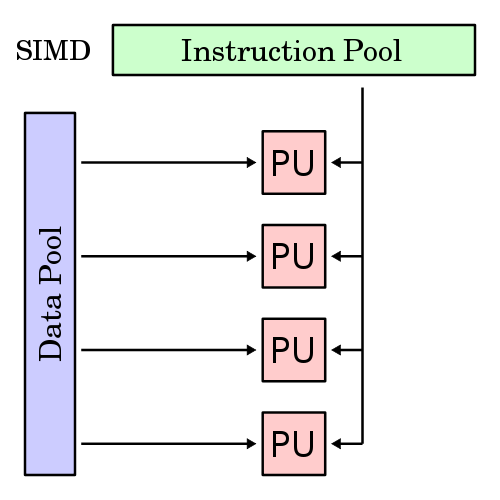
\includegraphics[width=0.4\textwidth]{images/simd.png}
\end{center}

Example: consider I ask people to erase boards in class...

Only works if we all do the same thing!

\end{frame}


%%%%%%%%%%%%%%%%%%%%%%%%%%%%%%%%%%%%%%%%%%%%%%%%%%%%%%%%%%%%%%%%%%%%%%%%%%%%%%%%
\begin{frame}[fragile]
  \frametitle{SIMD Example}

  
  Consider the following code:

\begin{lstlisting}[language=Rust]
pub fn foo(a: &[f64], b: &[f64], c: &mut [f64]) {
    for ((a, b), c) in a.iter().zip(b).zip(c) {
        *c = *a + *b;
    }
}\end{lstlisting}

    In this scenario, we have a regular operation over block data.\\[1em]

    We could use threads, but we'll use SIMD.

  
\end{frame}
%%%%%%%%%%%%%%%%%%%%%%%%%%%%%%%%%%%%%%%%%%%%%%%%%%%%%%%%%%%%%%%%%%%%%%%%%%%%%%%%

%%%%%%%%%%%%%%%%%%%%%%%%%%%%%%%%%%%%%%%%%%%%%%%%%%%%%%%%%%%%%%%%%%%%%%%%%%%%%%%%
\begin{frame}[fragile]
  \frametitle{SIMD Example---Assembly}

We can compile with \texttt{rustc} defaults
and get something like this as core loop contents:
\begin{verbatim}
  movsd   xmm0, qword ptr [rcx]
  addsd   xmm0, qword ptr [rdx]
  movsd   qword ptr [rax], xmm0
\end{verbatim}

This uses the SSE and SSE2 instructions
  
\end{frame}
%%%%%%%%%%%%%%%%%%%%%%%%%%%%%%%%%%%%%%%%%%%%%%%%%%%%%%%%%%%%%%%%%%%%%%%%%%%%%%%%


%%%%%%%%%%%%%%%%%%%%%%%%%%%%%%%%%%%%%%%%%%%%%%%%%%%%%%%%%%%%%%%%%%%%%%%%%%%%%%%%
\begin{frame}[fragile]
  \frametitle{SIMD Example---Assembly}

  If you additionally specify \texttt{-O}, the compiler generates a number of variants, including this middle one:
\begin{verbatim}
  movupd  xmm0, xmmword ptr [rdi + 8*rcx]
  movupd  xmm1, xmmword ptr [rdi + 8*rcx + 16]
  movupd  xmm2, xmmword ptr [rdx + 8*rcx]
  addpd   xmm2, xmm0
  movupd  xmm0, xmmword ptr [rdx + 8*rcx + 16]
  addpd   xmm0, xmm1
  movupd  xmmword ptr [r8 + 8*rcx], xmm2
  movupd  xmmword ptr [r8 + 8*rcx + 16], xmm0
\end{verbatim}

The \emph{packed} operations ({\tt p}) operate on multiple data
elements at a time.
\end{frame}
%%%%%%%%%%%%%%%%%%%%%%%%%%%%%%%%%%%%%%%%%%%%%%%%%%%%%%%%%%%%%%%%%%%%%%%%%%%%%%%%


\begin{frame}
\frametitle{SIMD}

The compiler uses SIMD instructions if the target architecture supports it.

We can explicitly invoke the instructions, or use libraries

It is complementary to using threads, and good for cases where loops operate over vectors of data.

SIMD instructions also work well on small data sets, where thread startup
cost is too high.

\end{frame}


%%%%%%%%%%%%%%%%%%%%%%%%%%%%%%%%%%%%%%%%%%%%%%%%%%%%%%%%%%%%%%%%%%%%%%%%%%%%%%%%
\begin{frame}
  \frametitle{SIMD Pros and Cons}

A more efficient (= less CPU resources) way to parallelize code than threads.

Data must be 16-byte aligned when loading to/storing from 128-bit registers.\\
\quad Not required in SSE4.2... if your CPU supports it.
  

\end{frame}
%%%%%%%%%%%%%%%%%%%%%%%%%%%%%%%%%%%%%%%%%%%%%%%%%%%%%%%%%%%%%%%%%%%%%%%%%%%%%%%%


\begin{frame}
\frametitle{Alignment}

\begin{center}
	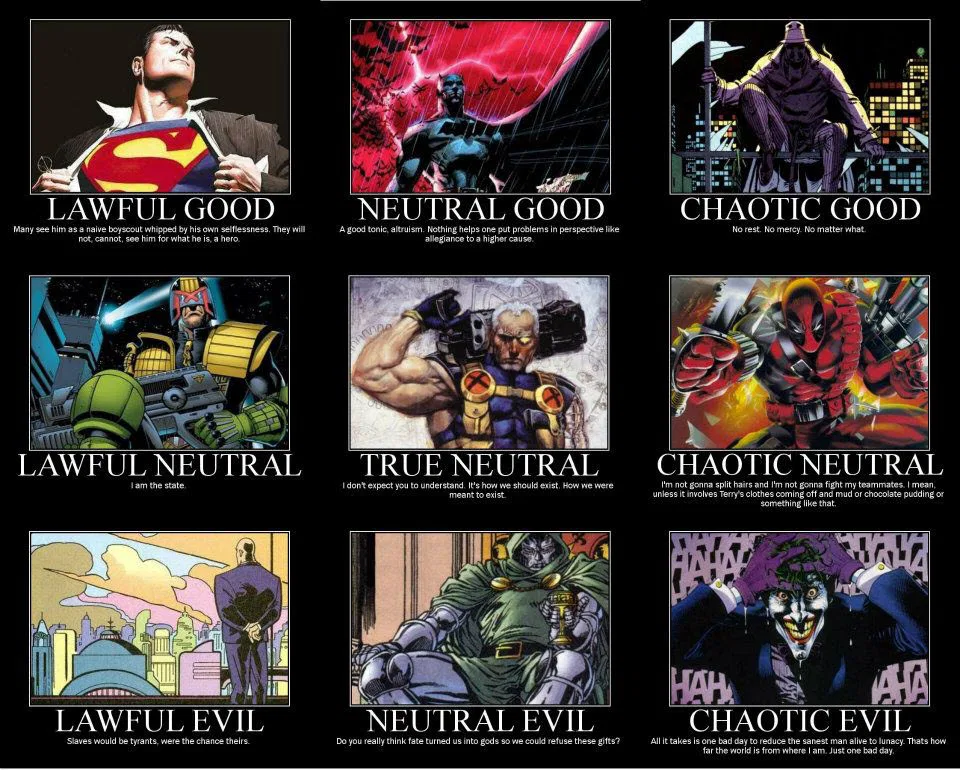
\includegraphics[width=0.8\textwidth]{images/superhero-alignment.png}
\end{center}

Oh. Not this kind of alignment.

\end{frame}



\begin{frame}
\frametitle{Forcing Alignment}

Rust will generally align primitives to their sizes. 

Under the default representation, Rust promises nothing else about alignment.

You can use the \texttt{repr(packed(N)} or \texttt{repr(align(N)} directives to express constraints on alignment.


\end{frame}


\begin{frame}[fragile]
\frametitle{Worked SIMD Example}

\begin{lstlisting}[language=Rust]
use simdeez::*;
use simdeez::scalar::*;
use simdeez::sse2::*;
use simdeez::sse41::*;
use simdeez::avx2::*;
simd_runtime_generate!(
// assumes that the input sizes are evenly divisible by VF32_WIDTH
pub fn add(a:&[f32], b: &[f32]) -> Vec<f32> {
  let len = a.len();
  let mut result: Vec<f32> = Vec::with_capacity(len);
  result.set_len(len);
  for i in (0..len).step_by(S::VF32_WIDTH) {
    let a0 = S::loadu_ps(&a[i]);
    let b0 = S::loadu_ps(&b[i]);
    S::storeu_ps(&mut result[0], S::add_ps(a0, b0));
  }
  result
});

fn main() {
  let a : [f32; 4] = [1.0, 2.0, 3.0, 4.0];
  let b : [f32; 4] = [5.0, 6.0, 7.0, 8.0];
  unsafe {
    println!("{:?}", add_sse2(&a, &b))
  }
}
\end{lstlisting}



\end{frame}



\begin{frame}
\frametitle{Single-Thread Performance}

``Can you run faster just by trying harder?''

\begin{center}

\includegraphics[width=0.7\textwidth]{images/theflash.jpg}
\end{center}

\end{frame}


\begin{frame}
\frametitle{Single-Thread Performance}


Performance improvements to date have \\
used parallelism
to improve throughput. 

Decreasing latency is trickier---\\
often requires domain-specific
tweaks. 

Today: one example of decreasing latency: \\
\hspace*{2em} Stream VByte.


\end{frame}


\begin{frame}
\frametitle{I have a cunning plan...}



Even Stream VByte uses parallelism:\\
\hspace*{2em}vector instructions. 

But there
are sequential improvements, \\
e.g. Stream VByte takes care to be predictable
for the branch predictor.


\end{frame}
\begin{frame}
\frametitle{Inverted Indexes (like it's CS 137 again!)}



\vspace*{-1em}
Abstractly: store a sequence of small integers.


Why Inverted indexes?

\hspace*{1cm}allow fast lookups by term;\\
\hspace*{1cm}support boolean queries combining terms.



\end{frame}
\begin{frame}
\frametitle{Dogs, cats, cows, goats. In ur documents.}


\begin{center}
\begin{tabular}{r|l}
docid & terms \\ \hline
1 & dog, cat, cow\\
2 & cat\\
3 & dog, goat\\
4 & cow, cat, goat\\
\end{tabular}
\end{center}


\end{frame}


\begin{frame}
\frametitle{Inverting the Index}


Here's the index and the inverted index:
\begin{center}
\begin{tabular}{r|l}
docid & terms \\ \hline
1 & dog, cat, cow\\
2 & cat\\
3 & dog, goat\\
4 & cow, cat, goat\\
\end{tabular} \hspace*{2em}
\begin{tabular}{r|l}
term & docs \\ \hline
dog & 1, 3 \\
cat & 1, 2, 4 \\
cow & 1, 4 \\
goat & 3, 4
\end{tabular}
\end{center}

Inverted indexes contain many small integers.

Deltas typically small if doc ids are sorted.


\end{frame}


\begin{frame}
\frametitle{Storing inverted index lists: VByte}


\vspace*{-2em}
VByte uses a variable number of bytes\\
to store integers.  

Why? Most integers are
small,\\
especially on today's 64-bit processors.

\end{frame}


\begin{frame}
\frametitle{How VByte Works}


VByte works like this:

\begin{itemize}
\item $x$ between 0 and $2^7-1$ (e.g. $17 = 0b10001$):\\
\hspace*{1em}$0xxx xxxx$, e.g. $0001 0001$;
\item $x$ between $2^7$ and $2^{14}-1$ (e.g. $1729 = 0b110 11000001$):\\
\hspace*{1em}                   $1xxx xxxx/0xxx xxxx$ (e.g. $1100 0001/0000 1101$);\\
\item $x$ between $2^{14}$ and $2^{21}-1$: \\
\hspace*{1em}$0xxx xxxx/1xxx xxxx/1xxx xxxx$;
\item etc.
\end{itemize}

Control bit, or high-order bit, is:\\
\hspace*{2em}0 once done representing the int,\\
\hspace*{2em}1 if more bits remain.


\end{frame}



\begin{frame}
\frametitle{Why VByte Helps}


Isn't dealing with variable-byte integers harder?\\
\hspace*{2em} $\bullet$~ Yup!

But perf improves: \\
\hspace*{2em} $\bullet$~  We are using fewer bits! 

We fit more information into RAM and
cache, and can get higher throughput. (think inlining)

Storing and reading 0s isn't good use of resources. 

However, a naive algorithm to decode VByte \\
gives branch mispredicts.

\end{frame}

\begin{frame}
\frametitle{Stream VByte}
\vspace*{-2em}

Stream VByte: a variant of VByte using SIMD.


Science is incremental. \\
Stream VByte builds on earlier work---\\
\hspace*{2em}masked VByte, {\sc varint}-GB, {\sc varint}-G8IU. 

Innovation in Stream VByte:\\
\hspace*{2em}\emph{store the control and data streams separately}.


\end{frame}

\begin{frame}
\frametitle{Control Stream}
\vspace*{-4em}

Stream VByte's control stream uses two bits per integer to represent the size of the integer:
\begin{center}
\vspace*{-3em}
\begin{tabular}{ll@{~~~~~~~~}ll}
00 & 1 byte & 10 & 3 bytes\\
01 & 2 bytes & 11 & 4 bytes
\end{tabular}
\end{center}


\end{frame}


\begin{frame}
\frametitle{Decoding Stream VByte}


Per decode iteration:\\
\hspace*{2em} reads 1 byte from the control stream,\\
\hspace*{2em} and 16 bytes of data.


Lookup table on control stream byte: decide how many
bytes it needs out of the 16 bytes it has read.

SIMD instructions: \\
\hspace*{2em}shuffle the bits each into their own integers. 

Unlike VByte, \\
Stream VByte uses all 8 bits
of data bytes as data.


\end{frame}



\begin{frame}
\frametitle{Stream VByte Example}


Say control stream contains $0b1000~1100$. \\
Then the data stream
contains the following sequence of integer sizes: $3, 1, 4, 1$. 

Out of the 16 bytes read,
this iteration uses 9 bytes; \\
\hspace*{2em} $\Rightarrow$ it advances the data pointer by 9. 

The SIMD
``shuffle'' instruction puts decoded integers from data stream at known positions in the
128-bit SIMD register.

Pad the first 3-byte integer with 1 byte, then
the next 1-byte integer with 3 bytes, etc. 

\end{frame}

\begin{frame}
\frametitle{Stream VByte: Shuffling the Bits}
\vspace*{-1em}

Say the data input is:\\
{\tt 0xf823~e127~2524~9748~1b..~....~....~....}. 

The 128-bit output is:\\
{\tt 0x00f8~23e1/0000~0027/2524 9748/0000~001b}\\
/s denote separation
between outputs. 

Shuffle mask is precomputed and
read from an array.

\end{frame}

\begin{frame}[fragile]
\frametitle{SIMD Instructions}

\vspace*{-1em}

The core of the implementation uses\\
three SIMD instructions:
\begin{lstlisting}[language=C]
  uint8_t C = lengthTable[control];
  __m128i Data = _mm_loadu_si128 ((__m128i *) databytes);
  __m128i Shuf = _mm_loadu_si128(shuffleTable[control]);
  Data = _mm_shuffle_epi8(Data, Shuf);
  databytes += C; control++;
\end{lstlisting}

\end{frame}


\begin{frame}
\frametitle{But Does It Work?!}

\vspace*{-1em}

Stream VByte performs better than previous techniques on a realistic input.


Why?

\begin{itemize}
\item control bytes are sequential:\\
\hspace*{1em} CPU can always prefetch the next control byte, \\
\hspace*{1em} because
its location is predictable;
\item data bytes are sequential \\
\hspace*{1em}and loaded at high throughput;
\item shuffling exploits the instruction set: \\
\hspace*{1em}takes 1 cycle;
\item control-flow is regular \\
\hspace*{1em}(tight loop which retrieves/decodes control
\& data;\\
\hspace*{1em}no conditional jumps).
\end{itemize}
\end{frame}


\end{document}

